\section{Protokół komunikacji bluetooth}
Robot Dark Explorer komunikuje się z otaczającym go światem przy użyciu
technologii Bluetooth. Zaimplementowany w oprogramowaniu robota protokół
komunikacji bazuje na ramce składającej się z 8 bitów nagłówka oraz 8 bitów
danych. Za pomocą informacji zawartych w nagłówku robot rozpoznaje
rodzaj akcji którą należy podjąć, natomiast po odczytaniu danych z kolejnego
przesłanego bajtu robot jest w stanie uruchomić odpowiedni wariant metody
zdefiniowanej w nagłówku przesłanej ramki. Jeżeli wysłane polecenie wymusza
odesłanie danych zwrotnych są one transmitowane przez robota w~postaci czystego
strumienia bajtów bez żadnych dodatkowych metadanych. 

\begin{figure}[h!]
 \centering
 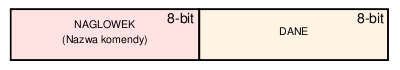
\includegraphics[height=18mm]{../images/ch05/old_req_schema.png}
 \caption{Schemat ramki komunikacyjej w pierwotnej wersji robota}
 \label{fig:OldCommFrame}
\end{figure}

Zaprezentowane tutaj podejście jest bardzo wydajne i nie ogranicza efektywnej
przepustowości łącza poprzez konieczność przesyłania dodatkowych danych
związanych z obsługą protokołu komunikacji. Nie mniej jednak tego rodzaju
komunikacja wymaga, od programisty tworzącego aplikacje klienckie, głębokiej
znajomości sposobu realizacji poszczególnych poleceń, tak aby mógł on
synchronizować komunikację zarówno pod względem czasowy jak i ilościowym. Kolejną
znaczącą niedogodnością jest fakt, iż bardzo często nawet najdrobnijesze zmiany w
oprogramowaniu robota wymuszają wprowadzanie zmian w aplikacji klienta pomimo
tego, że sposób wymiany komunikatów pozostał niezmieniony. Dotychczasowy sposób
wymiany danych nie gwarantował również mechanizmów wykrywania i zapobiegania
błędów transmisji na poziomie aplikacji. Wykorzystywany do komunikacji protokół
RFCOMM\footnote{Radio Frequency Communication} będący rozszerzeniem protokołu
L2CAP\footnote{Logical Link Control And Adaptation Protocol} gwarantuje nam
korekcję błędów na poziomie pakietów, niestety na poziomie aplikacji programista
musi samodzielnie wnioskować rozmiar prawdopodobnej odpowiedzi oraz kolejność
przeysłanych strumieni danych co w warunkach produkcyjnych może być czasami wręcz
niemożliwe.

Aby zaadresować wszystkie napotkane w czasie rozwoju robota problemy konieczne
okazało się zaprojektowanie nowego protokołu wartstwy aplikacji który ułatwiłby
tworzenie oprogramowania współpracującego z rozbudowaną wersją robota Dark
Explorer. Takim sposobem narodził się projekt protokołu komunikacji opartego o
ramki z 16 bitowym nagłówkiem. W ramach opracowanego standardu wyróżnić można
dwa rodzaje ramek. Do pierwszej grupy zaliczyć można ramki rządań wysyłane przez
urządzenia zewnętrzne w celu zlecenia robotowi wykonania manewru lub ropoczęcia
kolejnych etapów bardziej złożonej procedury. Diagram przedstawiający stukturę
funkcjonalną ramki rządania widoczny jest na rysunku \ref{fig:RfcommReqFrame}.

\begin{figure}[h!] 
 \centering
 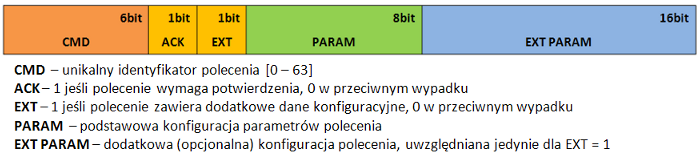
\includegraphics[width=\textwidth]{../images/ch05/req_schema2.png}
 \caption{Schemat funkcjonalny ramki komunikacyjej z rządaniem}
 \label{fig:RfcommReqFrame}
\end{figure}

Pierwsze 6 bitów zostało zarezerwowane na unikalny identyfikator polecenia które
robot ma wykonać. Pozwala to na zdefiniowanie 64 niezależnych funkcjonalnie
komend w ramach których, w wersji podstawowej, możliwe jest uruchomienie 256
niezależnych wariantów polecenia. W przypadku wykorzystania wersji rozszerzonej
nagłówka programista ma do dyspozycji 24 bity które może przeznaczyć na dane
polecenia i identyfikator podpolecenia w proporcjach odpowiadających wymaganiom
programisty. Kolejny bit nagłówka przeznaczony został na flagę potwierdzenia.
Umieszczenie 1 na wspomnianym bicie spowoduje iż robot po zakończeniu wykonywnia
rządania prześle ramkę potwierdzającą ze statusem wykonania akcji. Ułatwia to
programiście wykonywanie czynności sekwencyjnych takich jak np. wykonanie
zdjęcia za pomocą kamery i przesłanie go do aplikacji klienta. Ósmy bit nagłówka
zarezerwowany został na flagę z informacją o użyciu rozszerzonej wersji
nagłówka. Wymuszenie 1 na tym bicie spowoduje, że robot będzie oczekiwał na
dodatkowe 16 bitów danych rządania które mogą zostać wykorzystane do przesłania
bardziej skomplikowanej konfiguracji wykonania polecenia. Kolejne osiem bitów
stanowi tzw. podstawową konfigurację polecenia, która może służyć jako
identyfikator przy uruchamianiu odpowiedniego wariantu polecenia lub jako nośnik
danych potrzebnych do zrealizowania przesłanej komendy. W przypadku gdyby
rozmiar bufora konfiugracyjnego nie pozwalał na przechowanie wszystkich
wymaganych danych programista może wykorzystać dodatkowe 2 bajty konfiguracji
rozszrzonej.

Do drugiej grupy 


